\chapter{The Dataset}
\label{the_dataset}

\section{Motivation}

We have already motivated in Section \ref{sec:motivation} our desire to automatically generate documentation for individual elements of code: this would find great use as an IDE plugin for developers, whilst serving as a stepping stone for related tasks in code comprehension and type inference.
However, in order to examine the automatic documentation of individual elements of code, we require an appropriate dataset that, as demonstrated in Section \ref{sec:existing_datasets}, does not currently exist.

Therefore we set out to collect our own dataset, according to a number of criteria:

\begin{tight_enumerate}
    \item The data should be `real-world', ideally from open source code
    \item The data should have a close alignment between natural language and the code described. Ideally the natural language \textit{explicitly} describes the source code.
    \item The code used must be high quality and parsable, so that syntactic structure can be extracted.
    \item The data should require \textit{minimal} preprocessing and cleaning, to avoid mistakes and errors.
    \item The data should comparable in size to existing datasets
\end{tight_enumerate}

These goals were met in our collection of 40,000 function arguments with their respective natural language description, from 112 of the most popular libaries in `PyPI'\footnote{https://pypi.org/}, the Python Package Index - where open source python libraries are deployed. In the rest of this section we outline how we obtained this dataset, and the structure of the data within it. As this is a new and previously unseen dataset, we also present an analysis of its composition, both qualitatively and quantitatively.
Finally we present the different partitions of the dataset, we used in our experiments.


\section{Method of Collection} % (fold)
\label{sec:method_of_collection}

As mentioned in Section \ref{sub:python}, a number of conventions exist for the formatting of docstrings, the two most prominent ones being numpy-style and Google-style.
Not all codebases use such styles, (as seen in the Edinburgh Corpus \citep{barone_parallel_2017}), but they are popular with large open source projects. 

Sphinx\footnote{http://www.sphinx-doc.org/} is the industry standard for generating static HTML pages of documentation from source code. It contains a plugin - \textit{napoleon}\footnote{https://sphinxcontrib-napoleon.readthedocs.io/en/latest/} - especially designed for Python docstrings formatted according to the numpy or Google conventions. 
This plugin loads the source into memory and obtains the docstring from the AST itself.
Then \textit{napoleon} uses its custom parser to parse out different features from the docstring, such as argument names and their descriptions.

In order to make use of \textit{napoleon} docstring parsing facilities, we wrote a plugin, \textit{bonaparte}\footnote{https://github.com/condnsdmatters/bonaparte}, forking the \textit{napoleon} source. 
Instead of generating HTML, this plugin generated a series of yaml\footnote{http://yaml.org/} files with the associated data we required, including argument names, descriptions, docstrings, function code and filenames.
 

\begin{listing}[ht!]
\begin{minted}[fontsize=\footnotesize]{yaml}
-   argument_name: 'tensors'                                 
    argument_description: ' a list of variable or op tensors.'  
    function_name: 'add_zero_fraction_summaries'                
    function_args: ['tensors', 'prefix']                         
    function_signature: '(tensors, prefix=None)'                    
    library: 'tensorflow'                                
    filename: '/tensorflow/contrib/slim/python/slim/summaries.py'  
    other_argument_info:             
        'prefix': {desc: ' An optional prefix for the summary names.' }
    docstring: |
      Adds a scalar zero-fraction summary for each of the given tensors.

      :param tensors: a list of variable or op tensors.
      :param prefix: An optional prefix for the summary names.

      :returns: A list of scalar `Tensors` of type `string` whose contents are the
                 serialized `Summary` protocol buffer.
    src: |
      def add_zero_fraction_summaries(tensors, prefix=None):
        """<docstring>"""
        summary_ops = []
        for tensor in tensors:
          summary_ops.append(add_zero_fraction_summary(tensor, prefix=prefix))
        return summary_ops
\end{minted}
     \caption{An illustrative example of a single data point. The docstring in the source has been elided for brevity and replaced with the $<$docstring$>$ tag. A full table of the field names and types is presented in Appendix Table \ref{table:metadata}}
     \label{lst:single_point_short}
\end{listing}


Having written the plugin, we required a repository of large scale projects that documented their code according to these conventions. 
Therefore, we ran the bonaparte plugin on the 300 most popular libraries in PyPI, as of April 2018 \footnote{https://python3wos.appspot.com/}.
We then processed our data by removing arguments without descriptions (such as \mintinline[]{python}{self}) or without code bodies (from abstract base classes), or with an inappropriate documentation convention. 
This fulfilled our objective of obtaining a large number of arguments, descriptions and source code from popular high quality code-in-the-wild sources, with minimal processing to extract the relevant data.

\section{Structure of Data}

The dataset comprises of a list of Python function arguments, their natural language descriptions and surrounding metadata. 
This metadata is extensive, containing numerous fields including the source code of the function, function name and filename, among others. 
An example datapoint is presented in Listing \ref{lst:single_point_short}. The full structure of the data fields is also present in the appendix, Table \ref{table:metadata}. 


\section{Analysis of Data} % (fold)
\label{sec:analysis_of_data}

\subsection{Statistical Analysis of Libraries}

We first analysed our dataset by looking at the libraries included within it.
We found that although the criteria for choice of library was based solely on frequency of downloads from PyPI, there was a clear bias towards scientific libraries in the composition of the data.

Of the 112 libraries that eventually contributed data to the dataset, only 21 are labelled with the `Scientific/Engineering' tag on PyPI, yet these libraries contribute 68.3\% of arguments to the overall dataset, and 61.6\% of the functions. 
Even more surprisingly one library, \mintinline{python}{tensorflow}, contributes 41\% of the arguments to the data - vastly more than any other library.
In fact, as can be seen from Table \ref{table:breakdown_by_library}, it contributes almost six times as many arguments as the second placed library - coincidentally also developed by Google. 

\begin{table}[h!]
    \begin{center}
    \begin{tabular}{c | c | c | c}
        Library      & Arguments     & Functions  & Scientific \\
        \hline
        tensorflow   & $ 17002 $     & $ 4340 $ & True \\
        google   & $ 2829 $      & $ 1098 $ & False \\
        scipy    & $ 2030 $      & $ 549 $ & True \\
        networkx     & $ 1869 $      & $ 669 $ & True \\
        matplotlib   & $ 1457 $      & $ 366 $ & True \\
        sklearn      & $ 1403 $      & $ 368 $ & True \\
        pandas   & $ 1317 $      & $ 419 $ & True \\
        magenta      & $ 1045 $      & $ 357 $ & False \\
        (\textit{100 $<$ arguments $<$ 1000})   & $ 10172 $     & $ 3137 $ & True: 6, False: 26 \\
        (\textit{0 $<$ arguments $<$ 100})      & $ 2300 $      & $ 1036 $ & True: 9, False: 84 \\
        \hline
        \hline
        TOTAL    & $ 41424 $     & $ 12339 $ & True: 21, False: 112 \\
    \end{tabular}
    \caption {Break down of the largest libraries in the dataset, by contribution of arguments. Despite their relative infrequency in the overall dataset, scientific libraries contribute the majority of arguments and functions}
    \label{table:breakdown_by_library}
    \end{center}
\end{table}



This outsize contribution from relatively few libraries is largely the result of the design of these libraries and their use cases. 
Scientific libraries have vast APIs, and users of the libraries often require different interfaces for potentially similar functions. 
As an example, two library methods such as \mintinline{python}{conv2D} and \mintinline{python}{conv3D} may in an abstract sense perform very similar functions - a mathematical convolution - yet are critically distinct in a scientific setting.
The necessity of these kinds of distinctions, and the precision of their use case, leads these libraries to have large numbers of exposed functions, requiring clear documentation.

\begin{table}[h!]
    \begin{center}
    \begin{tabular}{c | c | c | c | c}
        & Top Argument Names & Count  &   Top Function Names & Count \\  
        \hline               
        1.   &  name     &     1917    &   fit       &    122 \\        
        2.   &  x        &     439     &   transform &    102 \\         
        3.   &  kwargs   &     303     &   train     &    77 \\         
        4.   &  axis     &     263     &   evaluate  &    71 \\        
        5.   &  dtype    &     260     &   get       &    61 \\         
        6.   &  a        &     230     &   conv2d    &    59 \\        
        7.   &  G        &     227     &   Client    &    52 \\        
        8.   &  inputs   &     224     &   update    &    46 \\        
        9.   &  input    &     223     &   add       &    45 \\         
        10.  &  value    &     210     &   specgram  &    45 \\         
    
    \end{tabular}
    \caption {The most popular variable names and function names in the raw dataset. As can be seen these are either dominated by scientific terms and single letter variable names, such as those in scientific libraries. Scientific functions which take large numbers of arguments contribute heavily to the dataset}
    \label{table:popular_variable_names}
    \end{center}
\end{table}

\subsection{Statistical Analysis of Arguments}

Corresponding to our findings on a library level, we found that a large number of function and argument names were very scientific in nature. Table \ref{table:popular_variable_names} illustrates this with a list of the most popular argument names and argument function names in the dataset.
\begin{table*}[p]
    \centering
\makebox[\linewidth][c]{


    \begin{tabular}{l r}

    \begin{tabular}{c | c }       
        Repetitions, $N$  & \shortstack{Names Repeated $N$ Times \\ (\% of Data) } \\
        \hline     
        1     &       11.74   \\          
        2 - 4 &       17.30       \\      
        5 - 9 &        10.99   \\          
        10 - 19 &      11.56   \\          
        20 - 99 &      26.12   \\          
        100 - 499 &     16.27   \\          
        500 - 1999 &      6.11  \\                

    \end{tabular}
    \quad
    \begin{tabular}{c | c  }       
        Repetitions, $N$  & \shortstack{Names Repeated $N$ Times \\ (\% of Unique Names)  } \\ 
        \hline     
        1     &     53.55      \\          
        2 - 4 &     31.15      \\          
        5 - 9 &       7.84      \\          
        10 - 19 &     3.96      \\          
        20 - 99 &     3.08      \\          
        100 - 499 &    0.41      \\          
        500 - 1999 &   0.02       \\                

    \end{tabular}
    \end{tabular}
}

        \caption { A table of the count and frequency of variable names as they feature in the raw dataset. Approximately half of all variables names occur over 10 times in the data. In particular a single outlier - the variable name \mintinline{python}{name} from \mintinline{python}{tensorflow}, accounts for 6.1\% of the collected data}
    \label{table:variable_histogram}



\makebox[\linewidth][c]{

    \begin{tabular}{l r}
    \begin{tabular}{c | c }       
        Repetitions, $N$  & \shortstack{(Name, Desc) Repeated $N$ Times \\ (\% of Data) } \\
        \hline     
        1 &               47.691  \\
        2 - 4 &           28.881 \\
        5 - 9 &            9.483 \\
        10 - 99 &         10.574 \\
        100 - 499 &        0.000 \\
        500 - 1999 &       3.371 \\    
                   

    \end{tabular}
    \quad
    \begin{tabular}{c | c  }       
        Repetitions, $N$  & \shortstack{(Name, Desc) Repeated $N$ Times \\ (\% of Unique (Name, Desc))  } \\ 
        \hline     
        1 &                77.009   \\
        2 - 4 &            19.561  \\
        5 - 9 &            2.472  \\
        10 - 99 &          0.953  \\
        100 - 499 &        0.000  \\
        500 - 1999 &       0.005  \\     
    \end{tabular}
    \end{tabular}
}
        \caption { A table of the count and frequency of as (name, description) pairs as they feature in the dataset. Although names are often repeated, a much greater fraction of data points have unique (name, description) pairs.}
    \label{table:name_desc_histogram}

\makebox[\linewidth][c]{

    \begin{tabular}{l r}
    \begin{tabular}{c | c }       
        Repetitions, $N$  & \shortstack{CodePaths Repeated $N$ Times \\ (\% of Paths) } \\
        \hline     
        1 &            2.195  \\     
        2 - 9 &           12.056  \\     
        10 - 99 &         22.349  \\      
        100 - 999 &       26.367    \\    
        1000 - 9999 &       30.418  \\     
        10000 - 99999 &          6.615   \\   

    \end{tabular}
    \quad
    \begin{tabular}{c | c  }       
        Repetitions, $N$  & \shortstack{CodePaths Repeated $N$ Times \\ (\% of Unique CodePaths)  } \\ 
        \hline     
        1 &        33.753    \\     
        2 - 9 &        51.099   \\     
        10 - 99 &      13.445   \\      
        100 - 999 &     1.510   \\    
        1000 - 9999 &     0.189   \\     
        10000 - 99999 &       0.005    \\   
    \end{tabular}
    \end{tabular}
}

        \caption { A table of the count and codepaths as they feature in the raw dataset. A larfe fraction of the datasets are repeated }
    \label{table:codepath_histogram} 


\end{table*}




Furthermore we found a lot of repetition of the same argument name within the dataset, as can be seen from the histogram in Table \ref{table:variable_histogram}.
Reassuringly we found that, aside from having different source code, these duplicates would also often have different descriptions and came from different packages.  A histogram of counts of unique (name, description) pairs verifies this in Table \ref{table:name_desc_histogram}, while some illustrative examples of the different descriptions and packages for the most popular names are presented in Appendix Tables \ref{table:descriptions_for_names} and \ref{table:packages_for_names}. 

We notice at this point that our distributions are heavily outweighed by one repeated (name, description), which accounts for 3.4\% of the whole data. This argument is from tensorflow: \mintinline[]{python}{name} - \textit{``a name for the operation (optional)"}. 
This outlier is visible too in our histogram of description lengths, (Figure \ref{fig:length_dist}), which otherwise shows a reasonable distribution of short descriptions. We note this outlier to inform our final preparations.  

Apart from this we note no major irregularities the arguments. The distribution of length of names is presented in Figure  \ref{fig:length_dist}, showing most are under 10 characters long.  We also note that the average number of arguments per function is a $3.836 \pm 2.96$, indicating that most most functions supply a modest number of arguments to the dataset.
\begin{figure}[tb]
    \centering
    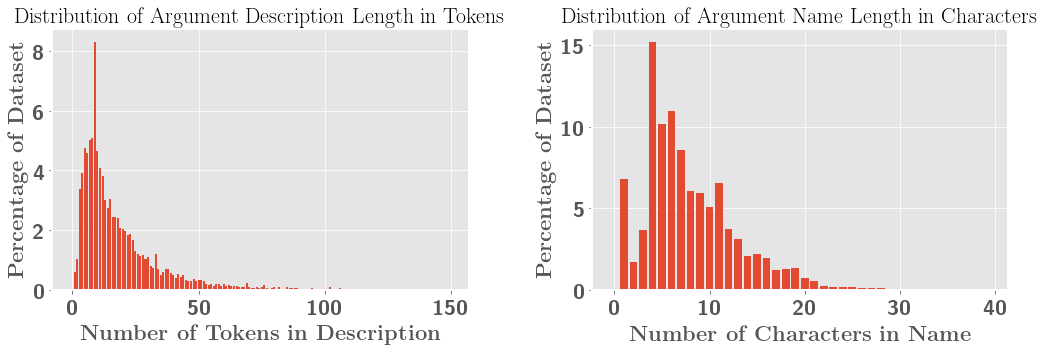
\includegraphics[width=\linewidth]{ImagesCodeRelated/length_distribution.png}
    \caption{Caption here}
    \label{fig:length_dist}
\end{figure}

\subsection{Statistical Analysis of Code} % (fold)
\label{sub:statistical_analysis_of_code}

Our dataset of derives from 264,056 lines of code (LOC)\footnote{Calculated with the \mintinline[]{python}{cloc} command line tool: https://github.com/AlDanial/cloc}.
When each function is split into different arguments, the total LOC associated with the dataset grows to 1,340,891. The distribution of these lengths is visible in figure \ref{fig:loc}, demonstrating that most functions are shorter than 50 lines of code.
The average length of the source code for a datapoint is 34 LOC, with a standard deviation of 57 LOC.

Since we aimed to investigate the code using \citet{alon_general_2018}'s path based parameterisation, we also investigated the most popular paths present in the dataset. Specfically, for each argument, we extracted the \textit{modified path-contexts} for which the argument was a terminal node, and counted the paths associated with these contexts.
A table histogram, Table \ref{table:codepath_histogram}, displays the distributions of paths. 
In it one can see that very few paths in the dataset are completely unique, which is promising if we are hoping to generalise across different sets of paths.
Furthermore, looking at the number of paths per data point (Table \ref{table:paths_per_point}), we see most data points have a large number of paths - about half have between 50 and 500 paths, which is also promising.

However, we also note from this table that some outliers have a preposterous large number of paths. These often correspond with the outliers that have exceptionally large line of code, and are often tied to items like class definitions. None-the-less, this indicates the data set is very much source from `real-life'.



\begin{figure}[tb]
    \centering
    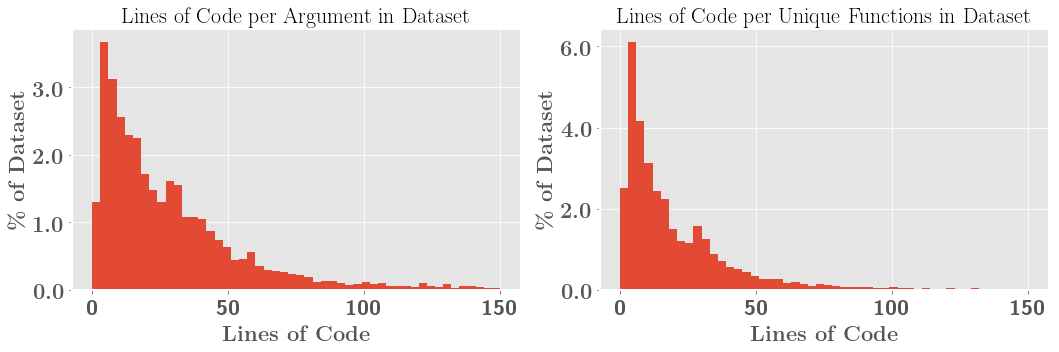
\includegraphics[width=\linewidth]{ImagesCodeRelated/lines_of_code.png}
    \caption{Caption here}
    \label{fig:loc}
\end{figure}



\begin{table}[p]
    \centering
    \begin{tabular}{c | c | c}       
    
           & Most Popular Paths  &  \% of Data \\  
        \hline
                
        1.  & Name $\uparrow$ keyword $\uparrow$ Call $\downarrow$ keyword &  0.679 \\ 
        2.  & Name $\uparrow$ Call $\downarrow$ Name &  0.672 \\ 
        3.  & Name $\uparrow$ keyword $\uparrow$ Call $\downarrow$ keyword $\downarrow$ Name &  0.647 \\ 
        4.  & Name $\uparrow$ Call $\downarrow$ Attribute &  0.296 \\ 
        5.  & Name $\uparrow$ Call $\downarrow$ Attribute $\downarrow$ Name &  0.241 \\ 
        6.  & Name $\uparrow$ keyword $\uparrow$ Call $\uparrow$ Assign $\uparrow$ If $\downarrow$ Assign $\downarrow$ Name &  0.229 \\ 
        7.  & Name $\uparrow$ AugAssign $\uparrow$ For $\uparrow$ FunctionDef $\downarrow$ Assign $\downarrow$ List $\downarrow$ List $\downarrow$ Num &  0.210 \\ 
        8.  & Name $\uparrow$ keyword $\uparrow$ Call $\uparrow$ Assign $\uparrow$ If $\downarrow$ Try $\downarrow$ Assign $\downarrow$ Call $\downarrow$ Name &  0.192 \\ 
        9.  & Name $\uparrow$ Call $\uparrow$ Assign $\uparrow$ Try $\uparrow$ If $\downarrow$ Assign $\downarrow$ Name &  0.189 \\ 
        10.  & Name $\uparrow$ Call $\uparrow$ Assign $\uparrow$ Try $\uparrow$ If $\downarrow$ Assign $\downarrow$ Call $\downarrow$ keyword &  0.184 \\ 
  
    \end{tabular}
    \caption { The most popular the paths of the the dataset. These only account for a very small amount of the data }
    \label{table:pop_paths} 
    \begin{tabular}{c | c | c  }       
    
        Paths Per DataPoint & Count  &  \%-ile of data points \\  
        \hline
        0 &               24  &     0.07865 \\
        1 &               138  &    0.53090 \\
        2 - 9 &           2451  &   8.56328 \\
        10 - 49 &         8717  &   37.13050 \\
        50 - 99 &         4517  &   51.93354 \\
        100 - 499 &       10023  &  84.78076 \\
        500 - 999 &       2449  &   92.80658 \\
        1000 - 9999 &     2160  &   99.88530 \\
        10000 - 99999 &   32  &     99.99017 \\
        100000 - 999999 & 3  &      100.00000 \\

    \end{tabular}
    \caption { A table of the count and frequency of distinct code paths as they feature in the raw dataset. 
        These can be either due to the repetition of function name throughout libraries, or by one argument contributing many functions }
    \label{table:paths_per_point} 

\end{table}


\section{Final Preparations} % (fold)
\label{sec:final_preparations}

Our final preparations of the dataset involved the filtering of duplicates that we had discovered in Section \ref{sec:analysis_of_data}, and creating two different partitionings of train, validation and test according to `in-project' splits and `out-project' splits.

First we restricted the number of duplicates of (name, description) pairs to 10. This removed the problem of exemplified by tensorflow's \mintinline[]{python}{name}, while still maintaining a 91\% of the data. This would be a \textbf{Full} dataset, which would be used to investigate AST related approaches, since the ASTs would be different for each of the duplicates.
We also prepared a \textbf{Reduced} dataset, where (name, description) pairs where unique. This would give us the opportunity, to do a broader analysis, where we might not use the AST.

Then we partitioned our datasets into train, validation and test in two different ways:
\begin{enumerate}
    \item \textbf{Random Split} - we partitioned the arguments randomly
    \item \textbf{Library Split} - we partitioned according to library, and choose library randomly
\end{enumerate}

In both cases we aimed to maintain a ratio of 7:1:2 for the train, validation and test. In the second case, the partition by library was not entirely random - due to its size, tensorflow was required to remain in training data, as too were some numpy and scipy, due to tensorflow's occasional use of their code. The rest of the libraries were chosen at random. This partition would allow us to investigate the difference of our algorithms in `in-project' and `out-of-project' situations.

Our final datasets are presented in Table \ref{tab:final_datasets}, with their train and validation splits.



\begin{table}[tb]
    \centering

    \begin{tabular}{c c c c}
    \hline
    Name       & Train & Validation & Test \\
    \hline
    \hline
    \textbf{Full Random Split}         & 24886 & 3551 & 7114 \\
    \textbf{Reduced Random Split}      & 16042 & 2289 & 4586\\
    \hline
    \hline
    \textbf{Full Library Split}         & 23969 & 3856 &7726 \\
    \textbf{Reduced Library Split}      & 15216 & 2565 & 5138 \\
    \hline
    \hline
    \end{tabular}
    \caption{Our Final Datasets}
    \label{tab:final_datasets}
\end{table}
